\documentclass{ieeeojies}
\usepackage{cite}
\usepackage{amsmath,amssymb,amsfonts}
\usepackage{algorithmic}
\usepackage{graphicx}
\usepackage{textcomp}
\usepackage{float}

\def\BibTeX{{\rm B\kern-.05em{\sc i\kern-.025em b}\kern-.08em
    T\kern-.1667em\lower.7ex\hbox{E}\kern-.125emX}}
% Đặt số trang ở bên trái


\markboth{right}{University of Information Technology}

\begin{document}
\title{Forecasting Index Prices Across the Three Stock Exchanges in Vietnam Using Statistical, Machine Learning, and Deep Learning Models}
\author{Tieu Thi Kieu Tien}
\corresp{Corresponding author: Tieu Thi Kieu Tien (e-mail: tieukieutien2000@gmail.com).}

\begin{abstract}
In current era, AI technology has made significant strides, with machine learning and deep learning algorithms proving instrumental in trend analysis and stock price predictions. The capabilities of AI offer investors valuable insights, enabling them to anticipate and understand market movements in advance. In this research article, we harness the power of machine learning and deep learning algorithms, specifically ARIMA, GRU, LSTM and SEQ2SEQ to forecast stock prices across three major indices in the Vietnamese stock market. The integration of these advanced algorithms empowers us to provide investors with a comprehensive tool set for predicting and navigating the dynamic landscape of stock market fluctuations
\end{abstract}

\begin{keywords}
{AI, Machine Learning, Deep Learning, Stock Market, ARIMA, GRU, LSTM, SEQ2EQ}
\end{keywords}

\titlepgskip=-15pt

\maketitle
\section{Introduction}
\label{sec:introduction}
The stock market, akin to a commodities marketplace, serves as a dynamic arena where individuals and businesses engage in trading, with shareholders and brokers comprising its clientele. Its primary purpose lies in facilitating private enterprises and governmental bodies in generating funds through the mechanisms of supply and demand. As companies evolve, the need for additional capital to support future endeavors becomes paramount. Following approval from existing shareholders, the issuance of new stocks allows companies to sell these shares to investors, thereby raising capital. The success of such endeavors contributes to the appreciation of stock market values for these shares.

Within the current investment landscape, two predominant strategies are long-term and short-term investments. Long-term investment involves the extended retention of shares, often spanning several years, while short-term strategies involve swift buying and selling processes. Investors engaging in short-term strategies typically execute transactions on a daily, hourly, or even minute-to-minute basis.

Amidst this financial complexity, various algorithms and techniques have emerged to aid in price prediction. In this paper, we delve into the application of a diverse array of models, including ARIMA, LSTM, GRU, SVR and SEQ2SEQ, to forecast stock prices for select corporations over the next 30 days

\section{RELATED WORK}
There are lots of research works in stock market prediction. Almost every data mining and prediction technique has been applied for predicting stock prices. Charity Egbunu, T.S Yange, and D.J Idoko used LSTM and RNN for forecasting the NIGERIA stock market and achieved an MSE of 0.1942, while RMSE shows 0.4990, 0.8300, and 0.8481 for the proposed RNN (LSTM)\cite{a7}. Another study by Dr. A S N Chakravarthy and Ashapu Bhavani focuses more on the Comparative Analysis between LSTM and GRU\cite{a6}. But when talking about details in explanation and implementation, Gaurang Sonkavde, Deepak Sudhakar Dharrao, Anupkumar M. Bongale, Sarika T. Deokate, Deepak Doreswamy, and Subraya Krishna Bhat explain LSTM, SVM, ARIMA, and GRU. This study explains in detail the step-by-step implementation, performance analysis, and provides a very clear direction for future research\cite{a5}.

\section{MATERIALS}
\subsection{DATASET}
In this research endeavor, our primary objective is to assess the accuracy of various machine learning models in predicting stock market indices in Vietnam. To accomplish this, we employed a dataset spanning over a decade, encompassing essential information on the historical price fluctuations and associated factors. The dataset from https://vn.investing.com and comprises crucial parameters such as:

\begin{itemize}
    \item Date : date of observation 
    \item Open : Opening price on the given day 
    \item High : Highest price on the given day
    \item Low : Lowest price on the given day 
    \item Close : Closing price on the given day 
    \item Vol : Volume of transactions on the given day
    \item Change\%: Percent changed on the given day
\end{itemize}

\begin{figure}[H]
    \centering
    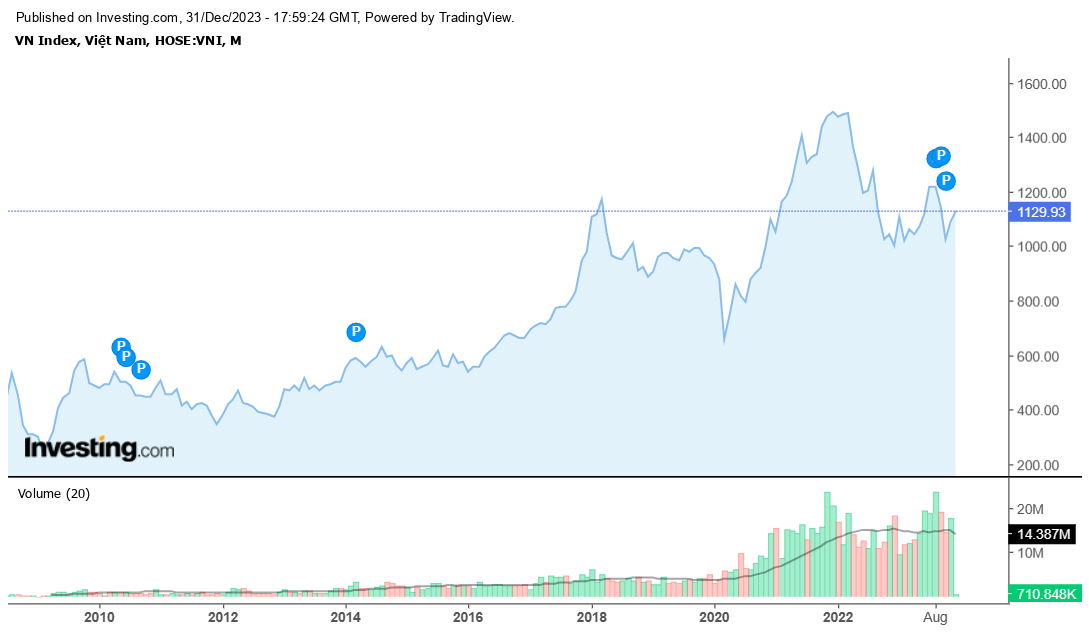
\includegraphics[width=0.8\linewidth]{VNI.PNG}
    \caption{VNIndex's price general chart}
    \label{fig:example}
\end{figure}

\subsubsection{VNIndex}
The VN-Index or Vietnam Stock Index is a capitalization-weighted index of all the companies listed on the Ho Chi Minh City Stock Exchange (HoSE) \cite{e3}

\begin{table}[H]
    \centering
    \begin{tabular}{|c|c|c|}
        \hline
          &  Open Price  \\
        \hline
        Count & 3483  \\
        \hline
        Mean & 780.35  \\
        \hline
        Min & 334.93 \\
        \hline
        Max &  1534.10\\
        \hline
        Q1 &  505.87\\
        \hline
        Q2 &  683.02\\
        \hline
        Q3 &  1002.875\\
        \hline
    \end{tabular}
    \caption{VNIndex summary data}
    \label{table:example}
\end{table}

\begin{figure}[H]
    \centering
    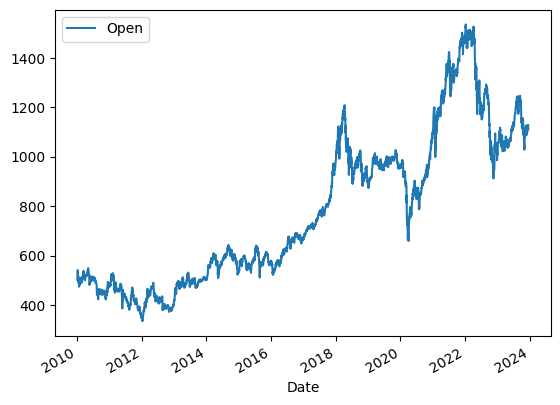
\includegraphics[width=0.8\linewidth]{VNI1.PNG}
    \caption{VNIndex's price from 2010 to 2023}
    \label{fig:example}
\end{figure}

\subsubsection{HNX Index}
HNX-Index is the index of all stocks traded at the Hanoi Stock Exchange (HNX). The HNX-Index can be called HASTC Index, because formerly the Hanoi Stock Exchange was also known as the Hanoi Stock Exchange Center (HASTC) \cite{e4}
\begin{table}[H]
    \centering
    \begin{tabular}{|c|c|c|}
        \hline
          &  Open Price  \\
        \hline
        Count & 3483  \\
        \hline
        Mean & 135.84  \\
        \hline
        Min & 50.63 \\
        \hline
        Max &  493.84\\
        \hline
        Q1 & 79.72\\
        \hline
        Q2 &  102.63\\
        \hline
        Q3 &  158.59\\
        \hline
    \end{tabular}
    \caption{HNX-Index summary data}
    \label{table:example}
\end{table}
\begin{figure}[H]
    \centering
    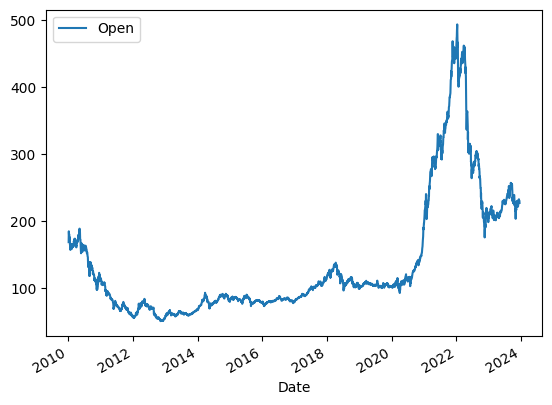
\includegraphics[width=0.8\linewidth]{HNX.PNG}
    \caption{VNIndex's price from 2010 to 2023}
    \label{fig:example}
\end{figure}
\subsubsection{UPCOM-Index}
UPCOM-Index is a stock index showing the price movement of all stocks on UPCOM, reflecting the capitalization value of companies listed on Upcom at the present time compared to the current value of shares \cite{e5}
\begin{table}[H]
    \centering
    \begin{tabular}{|c|c|c|}
        \hline
          &  Open Price  \\
        \hline
        Count & 3483  \\
        \hline
        Mean & 58.70  \\
        \hline
        Min & 28.8 \\
        \hline
        Max &  126.15\\
        \hline
        Q1 & 45.51\\
        \hline
        Q2 &  55.24\\
        \hline
        Q3 &  63.62\\
        \hline
    \end{tabular}
    \caption{Upcom-index summary data}
    \label{table:example}
\end{table}
\begin{figure}[H]
    \centering
    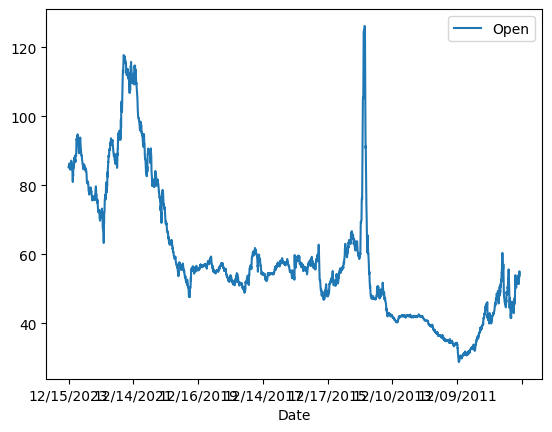
\includegraphics[width=0.8\linewidth]{UPC.PNG}
    \caption{Upcom-Index's price from 2010 to 2023}
    \label{fig:example}
\end{figure}

\subsection{MEASUREMENTS}
We use three three performance measures to evaluate the predictive performance such as:the mean squared error (MSE), the root mean square error (RMSE), the mean absolute error (MAE) and the mean absolute percentage error (MAPE). /\cite{e1}

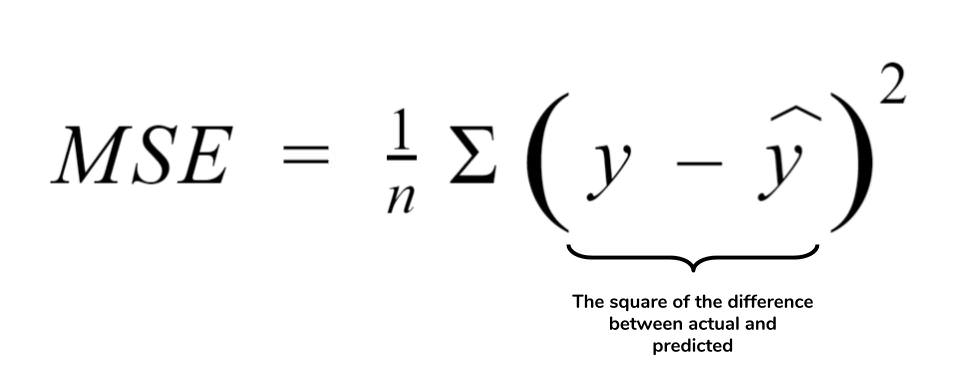
\includegraphics[width=0.47\textwidth]{MSE.jpg}
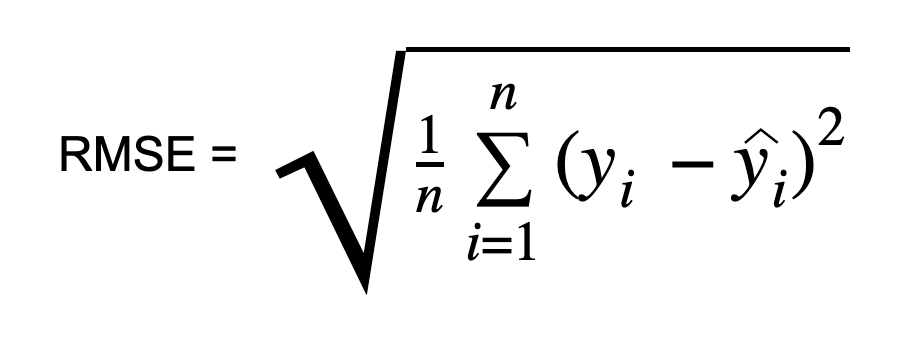
\includegraphics[width=0.47\textwidth]{RMSE.png}
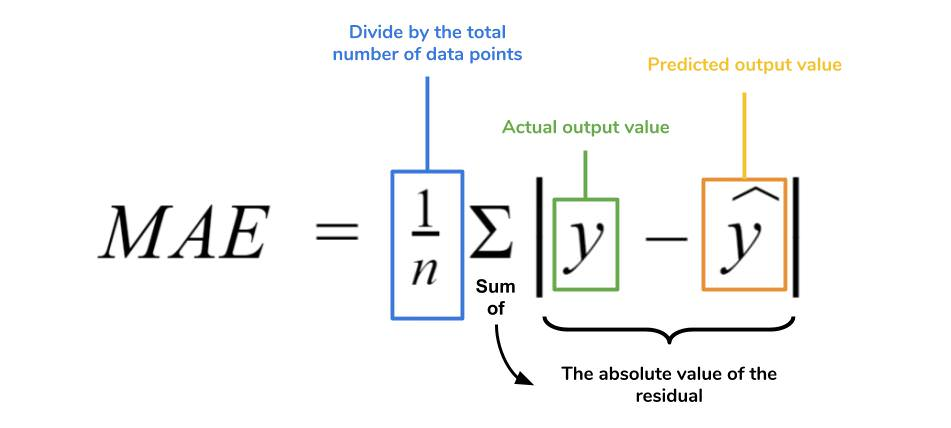
\includegraphics[width=0.47\textwidth]{MAE.jpg}
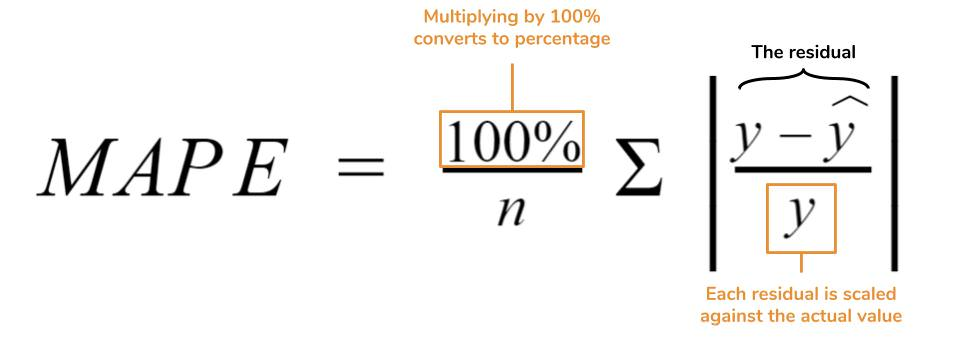
\includegraphics[width=0.47\textwidth]{MAPE.jpg}

\subsection{MODELINGS}
\subsubsection{linear model}
Linear regression, a fundamental statistical method, serves as a powerful tool for analyzing the relationship between a dependent variable and one or more independent variables. By fitting a linear equation to the observed data, this method allows for the estimation and prediction of outcomes based on the identified linear patterns, making it a widely used technique in various fields such as economics, finance, and social sciences.
Linear regression, a fundamental statistical method, serves as a powerful tool for analyzing the relationship between a dependent variable and one or more independent variables. By fitting a linear equation to the observed data, this method allows for the estimation and prediction of outcomes based on the identified linear patterns, making it a widely used technique in various fields such as economics, finance, and social sciences. \cite{a1}


\begin{equation}
y = \beta0 + \beta1X1
\end{equation}

\begin{itemize}
\item Y: The dependent variable.
\item X: The independent variable.
\item $\beta_0$: The intercept or the value of Y when other parameters equal zero.
\item $\beta_1$: The coefficient effect on X1. 
\end{itemize}

\subsubsection{ARIMA}
An Autoregressive integrated moving average (ARIMA), is a statistical analysis model that use analyzing and forecasting for time series data.
The ARIMA model have 3 important parameters:
p: The number of lags.
d: The number of times that the the raw data become stationary data.
q: The size of the moving average window.

\begin{equation}
    Y_t = c + \phi_1 Y_{t-1}  + \ldots + \phi_p Y_{t-p} + \varepsilon_t - \theta_1 \varepsilon_{t-1} - \ldots - \theta_q \varepsilon_{t-q}
\end{equation}

\subsubsection{GRUs}
GRU networks fall into the category of RNNs, i.e., neural networks whose underlying topology of inter-neuronal. GRUs was born to mitigate the problem of gradient vanishing of RNNs through gating mechanism.\cite{a3}
\begin{figure}[H]
    \centering
    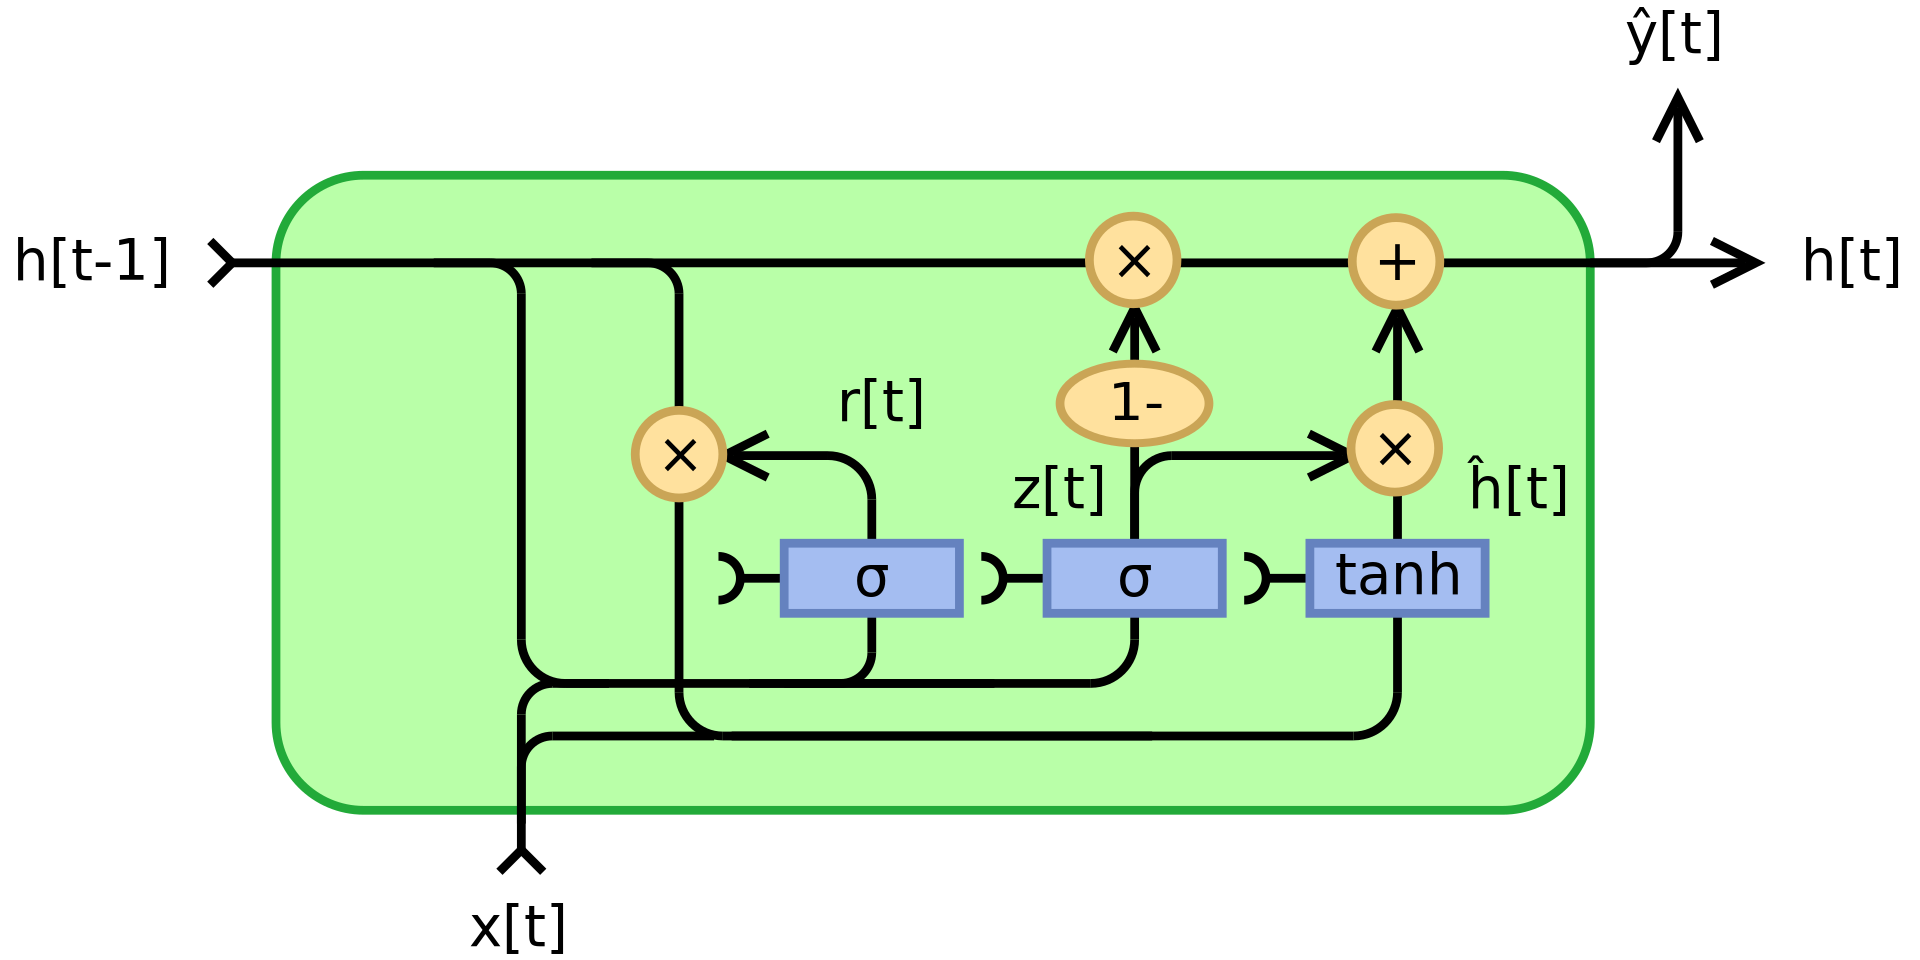
\includegraphics[width=0.8\linewidth]{GRU.PNG}
    \caption{GRU model fundamental.}
    \label{fig:example}
\end{figure}

\subsubsection{SVR}
Support Vector Regression (SVR) is a type of support vector machine (SVM), a supervised learning algorithm that can be used for classification or regression tasks. SVMs try to find the hyperplane in a high-dimensional space that maximally separates different classes or output values.
\begin{figure}[H]
    \centering
    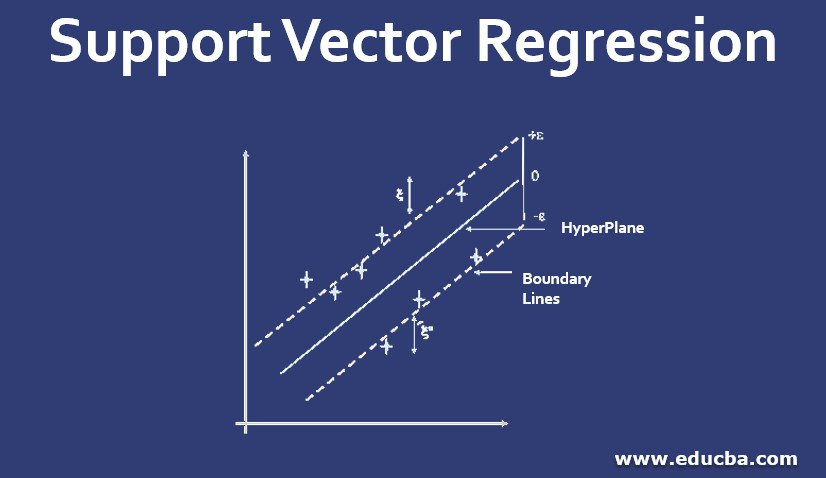
\includegraphics[width=0.8\linewidth]{SVR S.jpg}
    \caption{Caption}
    \label{fig:enter-label}
\end{figure}
\subsubsection{Long Short Term Memory Neural Network}
Long Short Term Memory Neural Network (LSTM) is also fall into the category of RNNs too. LSTM has feedback connections, i.e., it is capable of processing the entire sequence of data, apart from single data points such as images. This finds application in speech recognition, machine translation, etc. LSTM is a special kind of RNN, which shows outstanding performance on a large variety of problems.\cite{a4}

\begin{figure}[H]
    \centering
    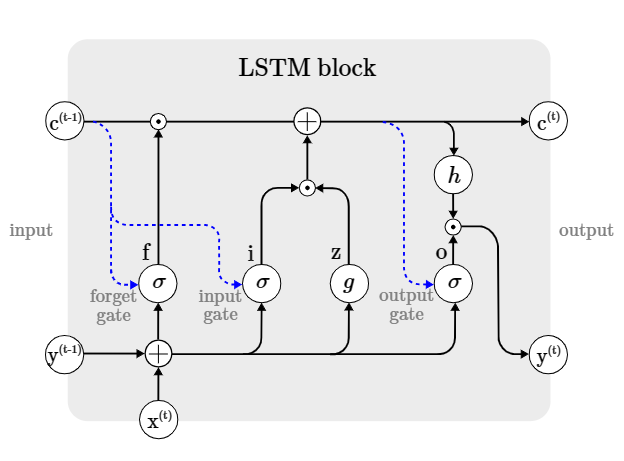
\includegraphics[width=0.8\linewidth]{LSTM.PNG}
    \caption{LSTM model fundamental.}
    \label{fig:example}
\end{figure}
\subsection{SEQ2SEQ}
Seq2Seq is network model for the time-series load forecasting. At each timestep, the encoder takes one series of data xt at time t, and its previous state ht1 and produces an output vector ht state and cell state Ct. The next decoder generates an output sequence yt, at each step taking at time t, the previous state, and a weighted combination of all the encoder outputs (i.e., encoder state vector) \cite{a4}
\begin{figure}[H]
    \centering
    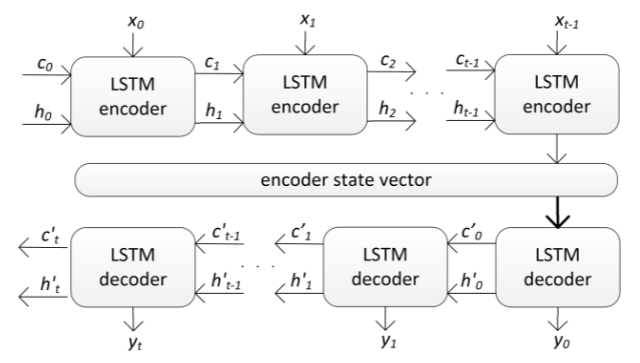
\includegraphics[width=0.8\linewidth]{Seq2seq.PNG}
    \caption{Seq2seq model fundamental}
    \label{fig:example}
\end{figure}

\section{RESULTS}

\subsection{VNIndex}
\subsubsection{Linear regression}
\begin{table}[H]
    \centering
    \begin{tabular}{|c|c|c|}
        \hline
         Measurement & Ratio &  Result  \\
        \hline
             & 7-3 & 155.70 \\
        MAE  & 8-2 & 190.3  \\
            & \textbf{9-1} & \textbf{163.68 }\\
        \hline
           & 7-3 & 38140.38  \\
        MSE  & 8-2 & 56083.57 \\
            & \textbf{9-1} & \textbf{31823.67 } \\
        \hline
           & 7-3 & 195.29 \\
        RMAE  & 8-2 & 236.81  \\
            & \textbf{9-1} & \textbf{178.39} \\
        \hline
           & 7-3 & 13.19  \\
        MAPE  & 8-2 & 14.45  \\
            & \textbf{9-1} & \textbf{15.25} \\
        \hline
    \end{tabular}
    \label{table:example}
\end{table}
\begin{figure}[H]
    \centering
    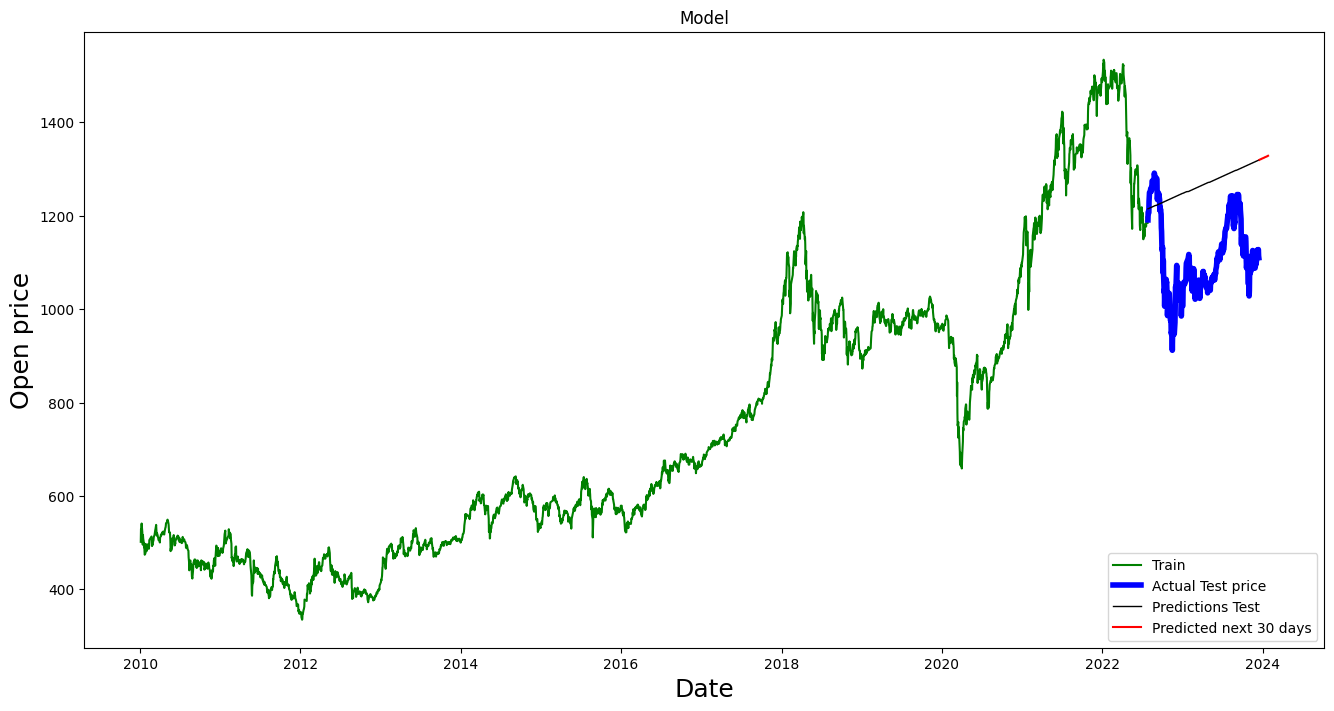
\includegraphics[width=0.8\linewidth]{RE VN DEX 91.jpg}
    \caption{The Linear Regression best modal for VNIndex}
    \label{fig:example}
\end{figure}

\subsubsection{ARIMA}
\begin{table}[H]
    \centering
    \begin{tabular}{|c|c|c|}
        \hline
         Measurement & Ratio &  Result  \\
        \hline
             & 7-3 & 10.79  \\
        MAE  & 8-2 & 11.26  \\
            & \textbf{9-1} & \textbf{10.11}  \\
        \hline
           & 7-3 & 239.10  \\
        MSE  & 8-2 & 245.63  \\
            & \textbf{9-1} & \textbf{196.08}  \\
        \hline
           & 7-3 & 15.46  \\
        RMAE  & 8-2 & 15.67  \\
            & \textbf{9-1} & \textbf{14.00}  \\
        \hline
           & 7-3 & 0.00  \\
        MAPE  & 8-2 & 0.00  \\
            & \textbf{9-1} & \textbf{0.00}  \\
        \hline
    \end{tabular}
    \label{table:example}
\end{table}
\begin{figure}[H]
    \centering
    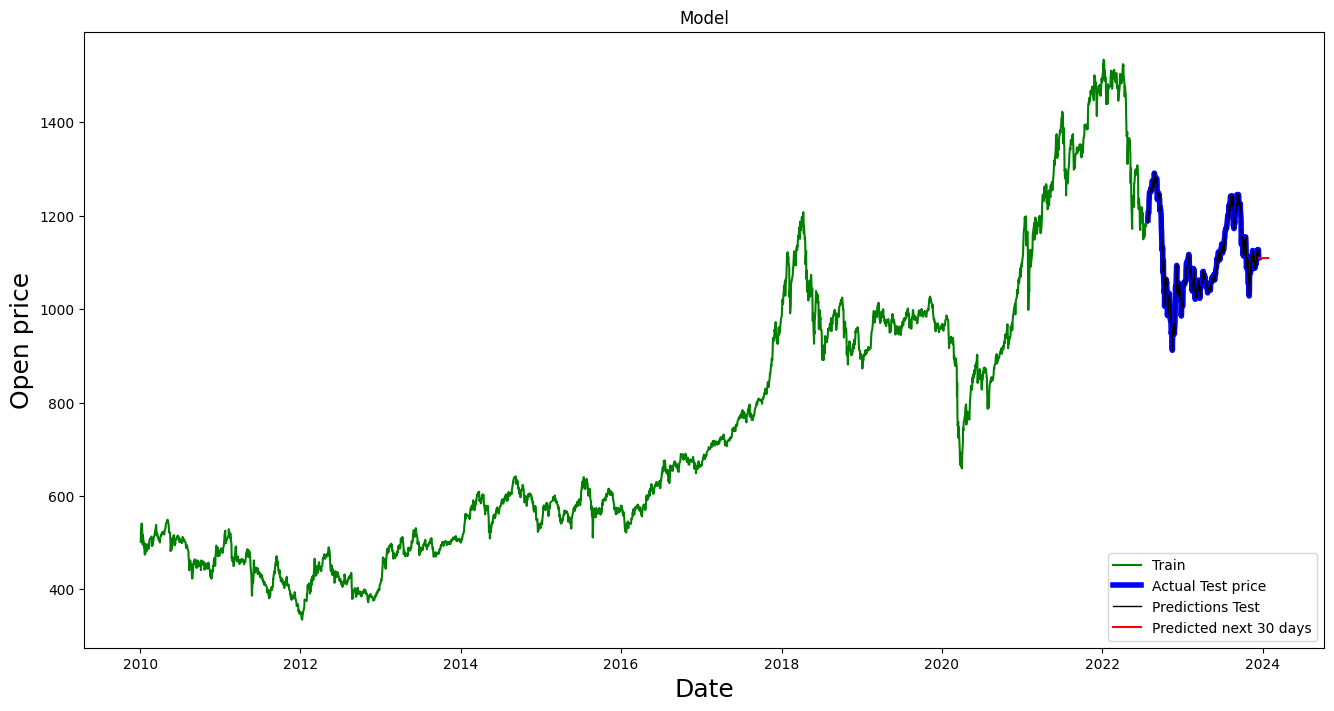
\includegraphics[width=0.8\linewidth]{ARIMA-VNI-.png}
    \caption{The ARIMA best modal for VNIndex}
    \label{fig:example}
\end{figure}

% =====

\subsubsection{GRU}
\begin{table}[H]
    \centering
    \begin{tabular}{|c|c|c|}
        \hline
         Measurement & Ratio &  Result  \\
        \hline
             & 7-3 & 1147.27  \\
        MAE  & 8-2 & 1224.39  \\
            & \textbf{9-1} &\textbf{ 1110.29}  \\
        \hline
           & 7-3 & 239.10  \\
        MSE  & 8-2 & 1525592.02  \\
            & \textbf{9-1} & \textbf{1236771.94}  \\
        \hline
           & 7-3 & 1356263.08  \\
        RMAE  & 8-2 & 1235.14  \\
            & \textbf{9-1} & \textbf{1112.10}  \\
        \hline
           & 7-3 & 1722.90  \\
        MAPE  & 8-2 & 1666.96  \\
            & \textbf{9-1} & \textbf{1722.06}  \\
        \hline
    \end{tabular}
    \label{table:example}
\end{table}
\begin{figure}[H]
    \centering
    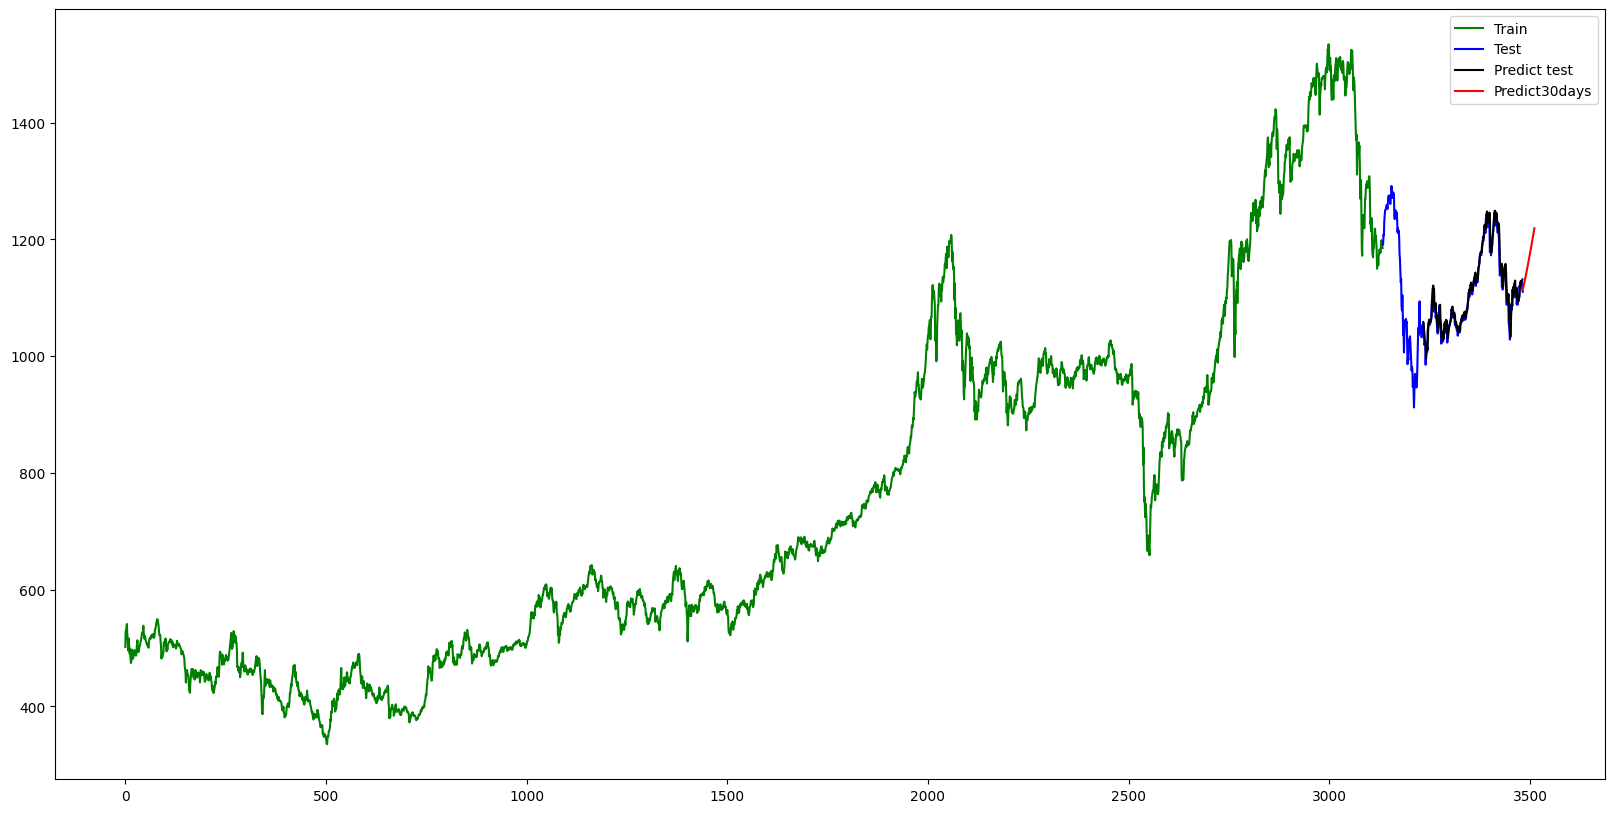
\includegraphics[width=0.8\linewidth]{gru-vni-91.png}
    \caption{The GRU best modal for VNIndex}
    \label{fig:example}
\end{figure}
% =====
\subsubsection{SVR}
\begin{table}[H]
    \centering
    \begin{tabular}{|c|c|c|c|}
        \hline
         Measurement & Ratio &  Result  \\
        \hline
             & 7-3 & 279.31 \\
        MAE  & 8-2 & 348.98  \\
            & \textbf{9-1} & \textbf{17.05} \\
        \hline
           & 7-3 & 149604.43  \\
        MSE  & 8-2 & 185599.56 \\
            & \textbf{9-1} & \textbf{705.19}  \\
        \hline
           & 7-3 & 386.78 \\
        RMAE  & 8-2 & 430.81  \\
            & \textbf{9-1} &\textbf{ 26.55} \\
        \hline
           & 7-3 & 0.21  \\
        MAPE  & 8-2 & 0.26  \\
            & \textbf{9-1} & \textbf{0.01} \\
        \hline
    \end{tabular}
    \label{table:example}
\end{table}
\begin{figure}[H]
    \centering
    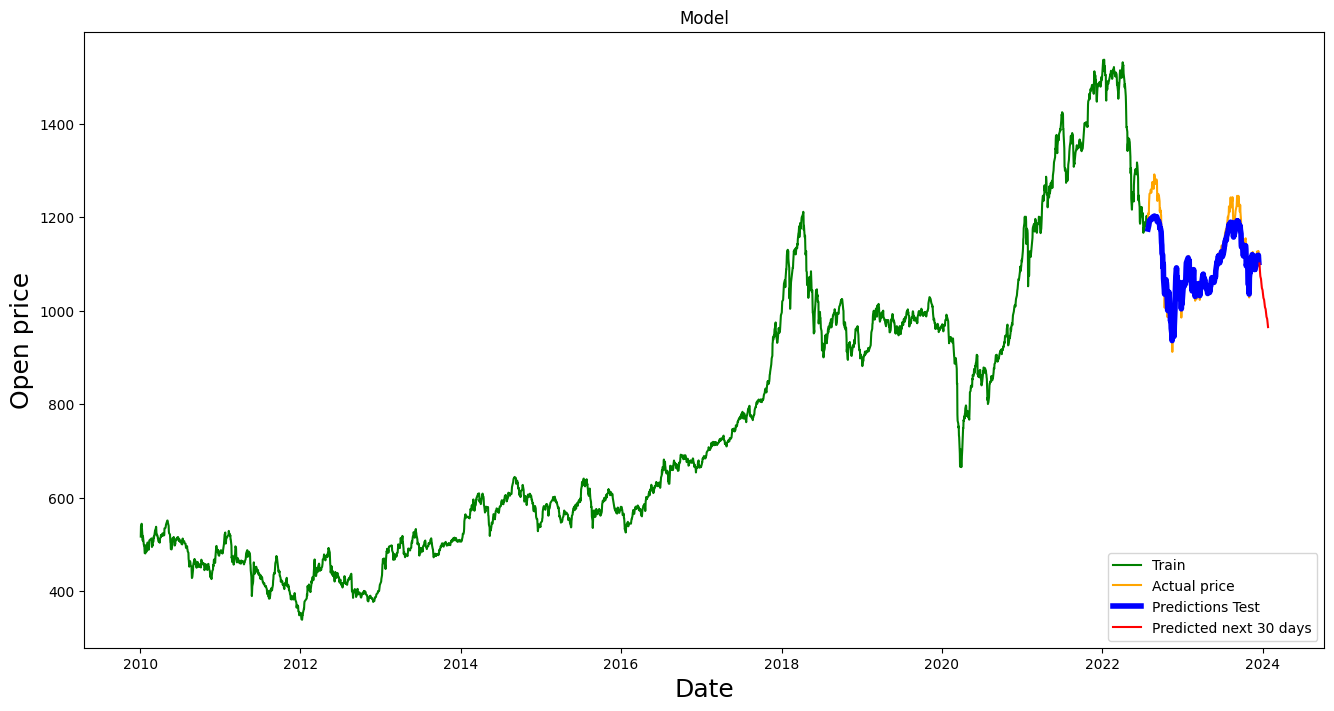
\includegraphics[width=0.8\linewidth]{SVR VN 91.jpg}
    \caption{The SVR best modal for VNIndex}
    \label{fig:example}
\end{figure}

\subsubsection{LSTM}
\begin{table}[H]
    \centering
    \begin{tabular}{|c|c|c|}
        \hline
         Measurement & Ratio &  Result  \\
        \hline
             & 7-3 & 63.37  \\
        MAE  & 8-2 & 66.53  \\
            & \textbf{9-1 }& \textbf{31.93}  \\
        \hline
           & 7-3 & 6837.14  \\
        MSE  & 8-2 & 6788.03  \\
            & \textbf{9-1} & \textbf{2029.33}  \\
        \hline
           & 7-3 & 82.68  \\
        RMAE  & 8-2 & 82.38  \\
            & \textbf{9-1} & \textbf{45.04 } \\
        \hline
           & 7-3 & 0.05  \\
        MAPE  & 8-2 & 0.05  \\
            & \textbf{9-1} &\textbf{ 0.02 } \\
        \hline
    \end{tabular}
    \label{table:example}
\end{table}
\begin{figure}[H]
    \centering
    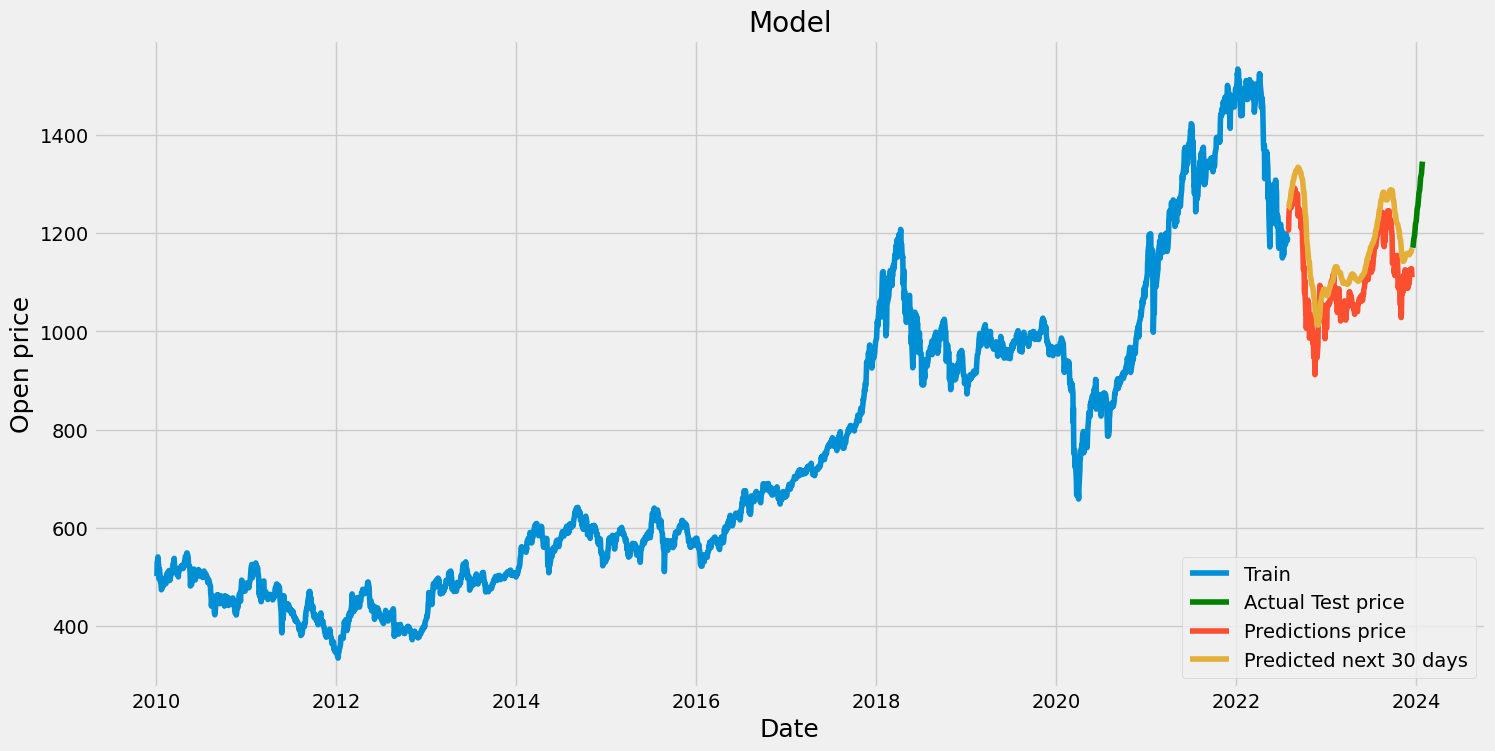
\includegraphics[width=0.8\linewidth]{LM VNI 91.jpg}
    \caption{The LSTM best modal for VNIndex}
    \label{fig:example}
\end{figure}
% ======
\subsubsection{SEQ2SEQ}
\begin{table}[H]
    \centering
    \begin{tabular}{|c|c|c|}
        \hline
         Measurement & Ratio &  Result  \\
        \hline
             & \textbf{7-3} & \textbf{6.39} \\
        MAE  & 8-2 & 6.45  \\
            & 9-1 & 7.86 \\
        \hline
           &\textbf{ 7-3} & \textbf{82.83}  \\
        MSE  & 8-2 & 94.11 \\
            & 9-1 & 135.97  \\
        \hline
           & \textbf{7-3} & \textbf{9.10} \\
        RMAE  & 8-2 & 9.70  \\
            & 9-1 & 11.66 \\
        \hline
           & \textbf{7-3} & \textbf{0.10}  \\
        MAPE  & 8-2 & 0.00  \\
            & 9-1 & 0.01 \\
        \hline
    \end{tabular}
    \label{table:example}
\end{table}

\begin{figure}[H]
    \centering
    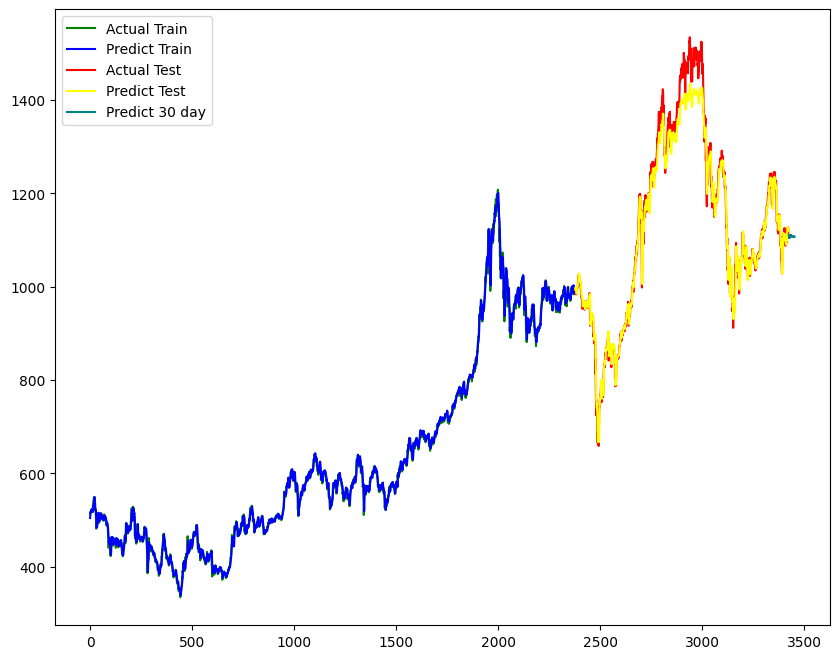
\includegraphics[width=0.8\linewidth]{SE VNI 73.jpg}
    \caption{The SEQ2SEQ best modal for VNIndex}
    \label{fig:example}
\end{figure}

\subsection{HNX-Index}
\subsubsection{Linear regression}
\begin{table}[H]
    \centering
    \begin{tabular}{|c|c|c|}
        \hline
         Measurement & Ratio &  Result  \\
        \hline
             & 7-3 & 17.76 \\
        MAE  & 8-2 & 178.14 \\
            & \textbf{9-1} & \textbf{19.40} \\
        \hline
           & 7-3 & 505.04  \\
        MSE  & 8-2 & 38736.97 \\
            & \textbf{9-1} &\textbf{ 846.46}  \\
        \hline
           & 7-3 & 22.40 \\
        RMAE  & 8-2 & 196.81  \\
            & \textbf{9-1} & \textbf{29.09} \\
        \hline
           & 7-3 & 19.98  \\
        MAPE  & 8-2 & 57.65  \\
            & \textbf{9-1} &\textbf{ 7.93} \\
        \hline
    \end{tabular}
    \label{table:example}
\end{table}
\begin{figure}[H]
    \centering
    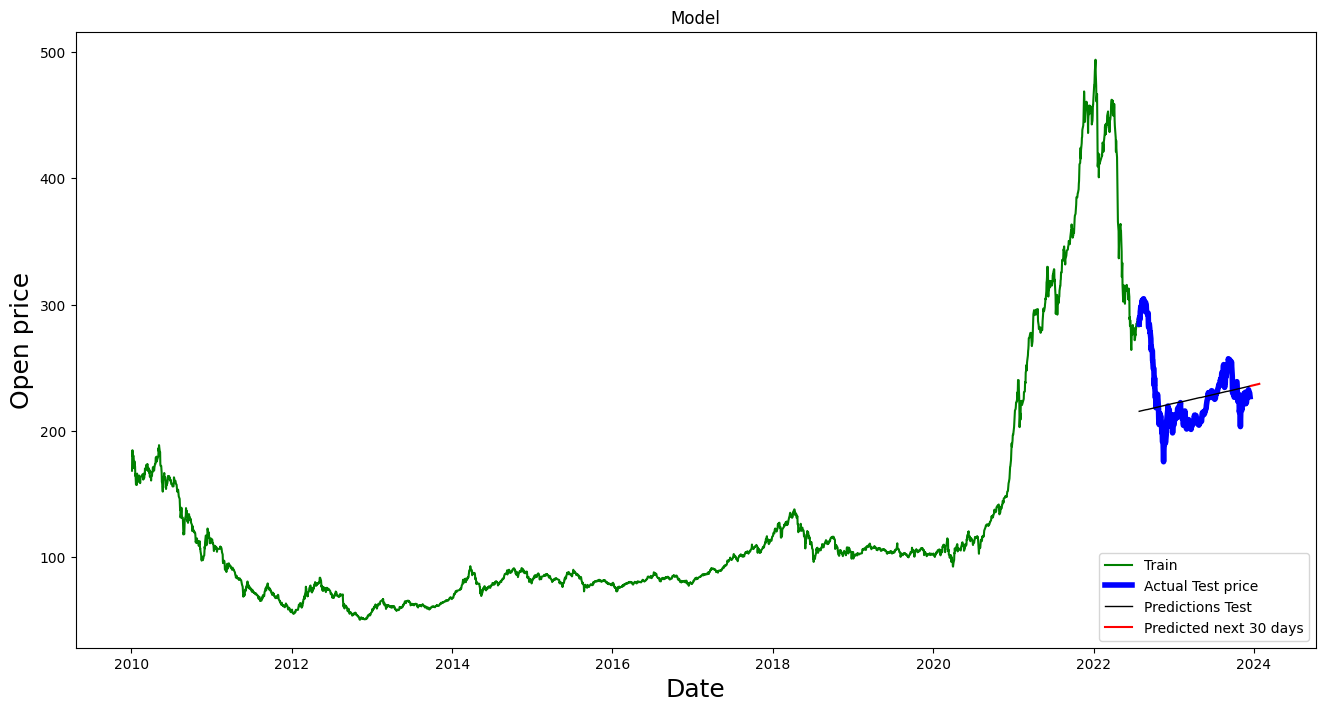
\includegraphics[width=0.8\linewidth]{LINEAR HNX91.jpg}
    \caption{The Linear Regression best modal for HNX-Index}
    \label{fig:example}
\end{figure} 



\subsubsection{ARIMA}
\begin{table}[H]
    \centering
    \begin{tabular}{|c|c|c|}
        \hline
         Measurement & Ratio &  Result  \\
        \hline
             & 7-3 & 2.81  \\
        MAE  & 8-2 & 3.41  \\
            & \textbf{9-1} & \textbf{2.49}  \\
        \hline
           & 7-3 & 18.00  \\
        MSE  & 8-2 & 23.85  \\
            & \textbf{9-1} & \textbf{12.34}  \\
        \hline
           & 7-3 & 4.25  \\
        RMAE  & 8-2 & 4.88  \\
            & \textbf{9-1} & \textbf{3.51}  \\
        \hline
           & 7-3 & 0.01  \\
        MAPE  & 8-2 & 0.01  \\
            & \textbf{9-1} & \textbf{0.01}  \\
        \hline
    \end{tabular}
    \label{table:example}
\end{table}
\begin{figure}[H]
    \centering
    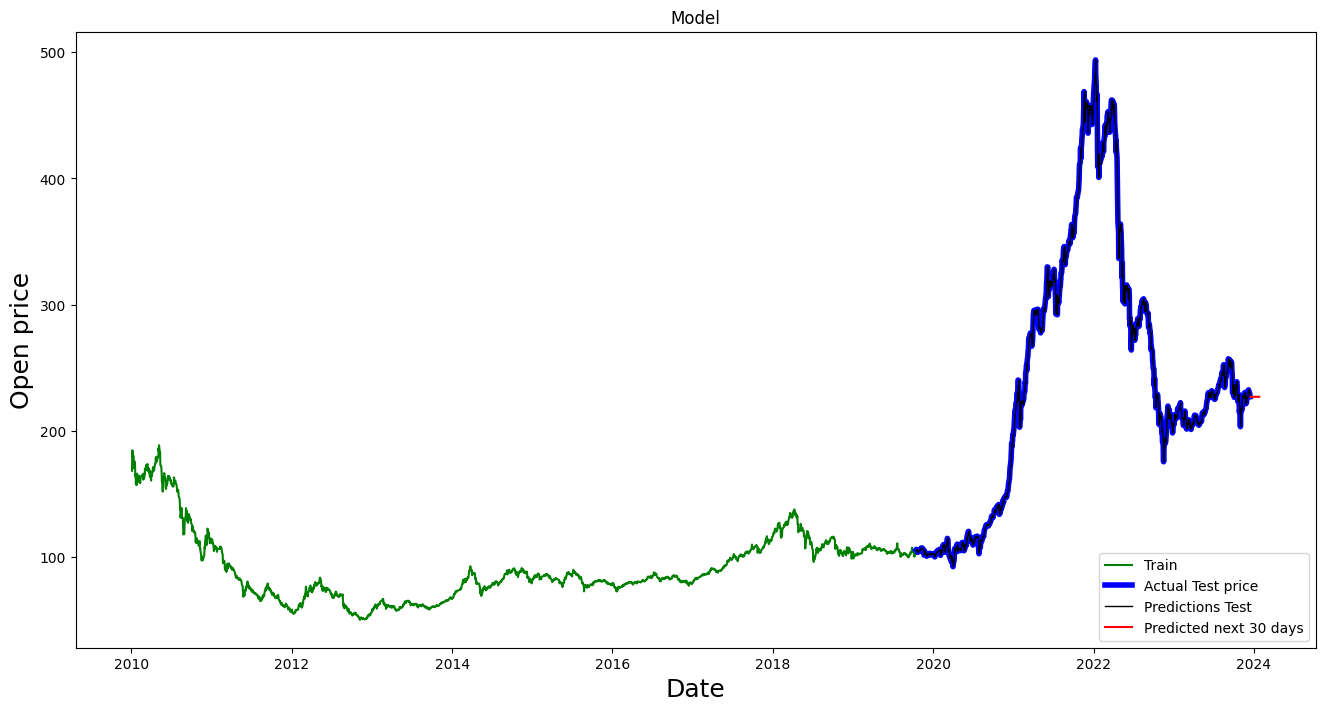
\includegraphics[width=0.8\linewidth]{A91.jpg}
    \caption{The ARIMA best modal for HNX-Index}
    \label{fig:example}
\end{figure} 
\subsubsection{GRU}
\begin{table}[H]
    \centering
    \begin{tabular}{|c|c|c|}
        \hline
         Measurement & Ratio &  Result  \\
        \hline
             & \textbf{7-3} & \textbf{10.79}  \\
        MAE  & 8-2 & 295.18  \\
            & {9-1} & {222.92}  \\
        \hline
           & \textbf{7-3} & \textbf{239.10}  \\
        MSE  & 8-2 & 95183.85  \\
            & {9-1} & {49900.74}  \\
        \hline
           & \textbf{7-3} & \textbf{15.46}  \\
        RMAE  & 8-2 & 308.51  \\
            & {9-1} & {223.38}  \\
        \hline
           & \textbf{7-3} &\textbf{ 0.00}  \\
        MAPE  & 8-2 & 550.80  \\
            & {9-1} & {573.87}  \\
        \hline
    \end{tabular}
    \label{table:example}
\end{table}
\begin{figure}[H]
    \centering
    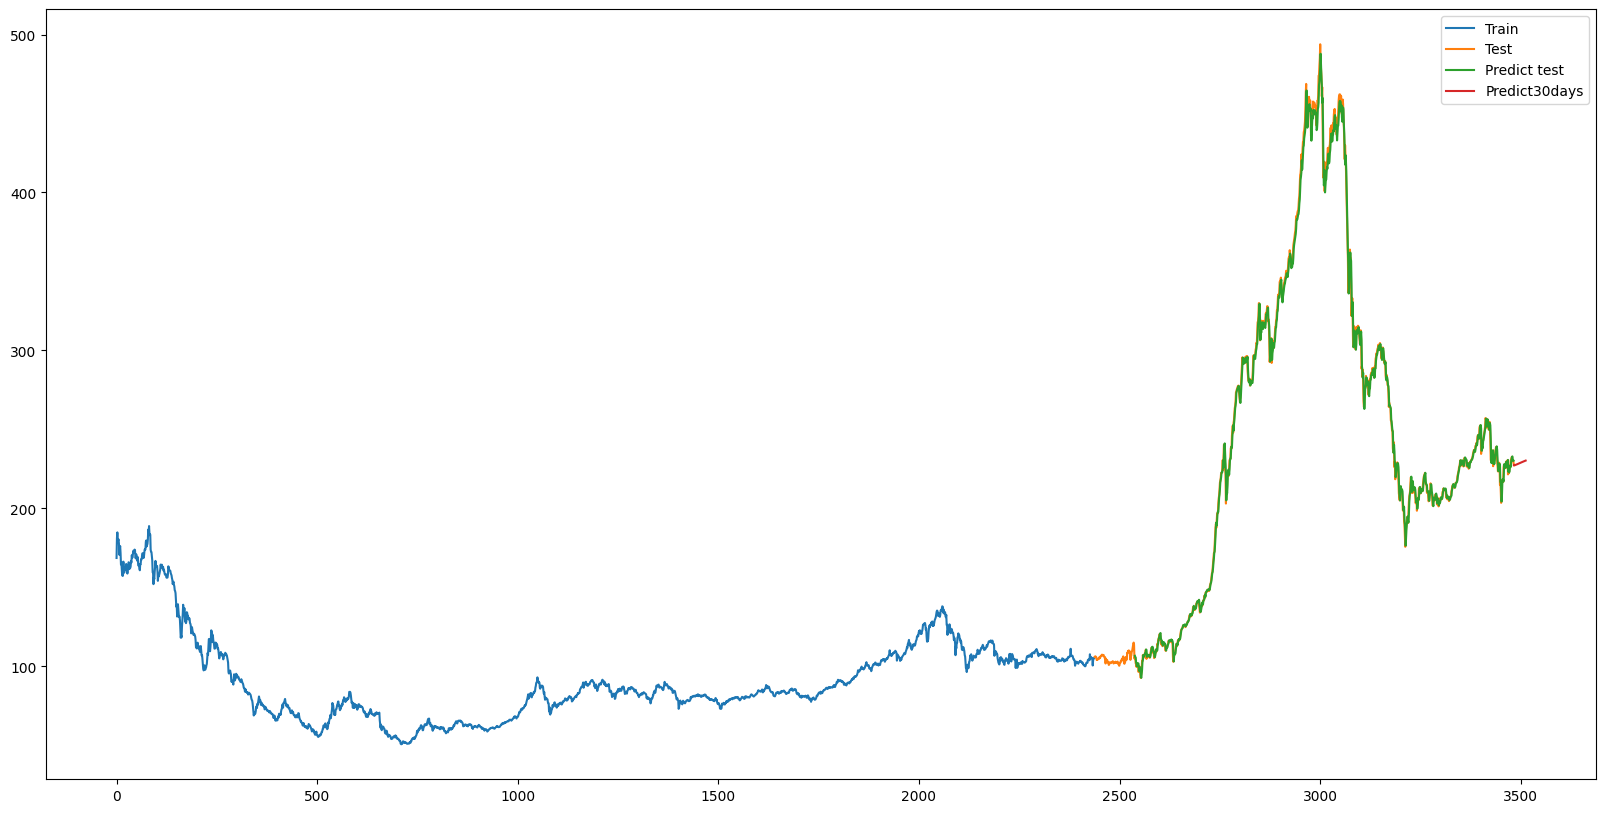
\includegraphics[width=0.8\linewidth]{GRU-HNX-73.png}
    \caption{The GRU best modal for HNX-Index}
    \label{fig:example}
\end{figure}
\subsubsection{SVR}
\begin{table}[H]
    \centering
    \begin{tabular}{|c|c|c|}
        \hline
         Measurement & Ratio &  Result  \\
        \hline
             & 7-3 & 123.57 \\
        MAE  & 8-2 & 147.27  \\
            & \textbf{{9-1}} & \textbf{{1.43}} \\
        \hline
           & 7-3 & 26541.66  \\
        MSE  & 8-2 & 31584.99 \\
            & \textbf{{9-1}} & \textbf{{3.18}}  \\
        \hline
           & 7-3 & 165.91 \\
        RMAE  & 8-2 & 177.72  \\
            & \textbf{{9-1}} & \textbf{{1.78}} \\
        \hline
           & 7-3 & 0.40  \\
        MAPE  & 8-2 & 0.44  \\
            & \textbf{{9-1}} & \textbf{{0.00}} \\
        \hline
    \end{tabular}
    \label{table:example}
\end{table}
\begin{figure}[H]
    \centering
    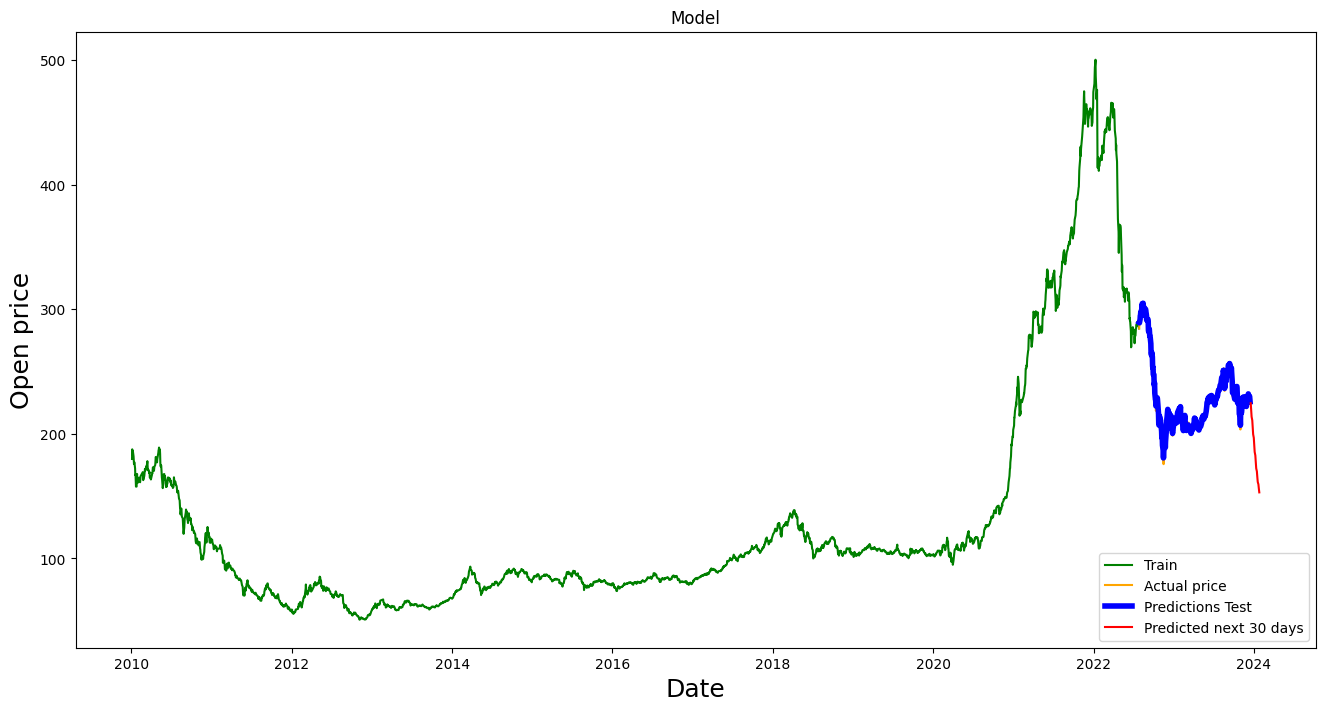
\includegraphics[width=0.8\linewidth]{SVR HNX 91.jpg}
    \caption{The SVR best modal for HNX-Index}
    \label{fig:example}
\end{figure}

\subsubsection{LSTM}
\begin{table}[H]
    \centering
    \begin{tabular}{|c|c|c|}
        \hline
         Measurement & Ratio &  Result  \\
        \hline
             & 7-3 & 18.74  \\
        MAE  & 8-2 & 49.36  \\
            & \textbf{9-1} & \textbf{16.34}  \\
        \hline
           & 7-3 & 792.75  \\
        MSE  & 8-2 & 5300.61  \\
            & \textbf{9-1} & \textbf{336.68}  \\
        \hline
           & 7-3 & 28.15  \\
        RMAE  & 8-2 & 72.80  \\
            & \textbf{9-1} &\textbf{ 19.14}  \\
        \hline
           & 7-3 & 0.06  \\
        MAPE  & 8-2 & 0.13  \\
            & \textbf{9-1 }& \textbf{0.07}  \\
        \hline
    \end{tabular}
    \label{table:example}
\end{table}
\begin{figure}[H]
    \centering
    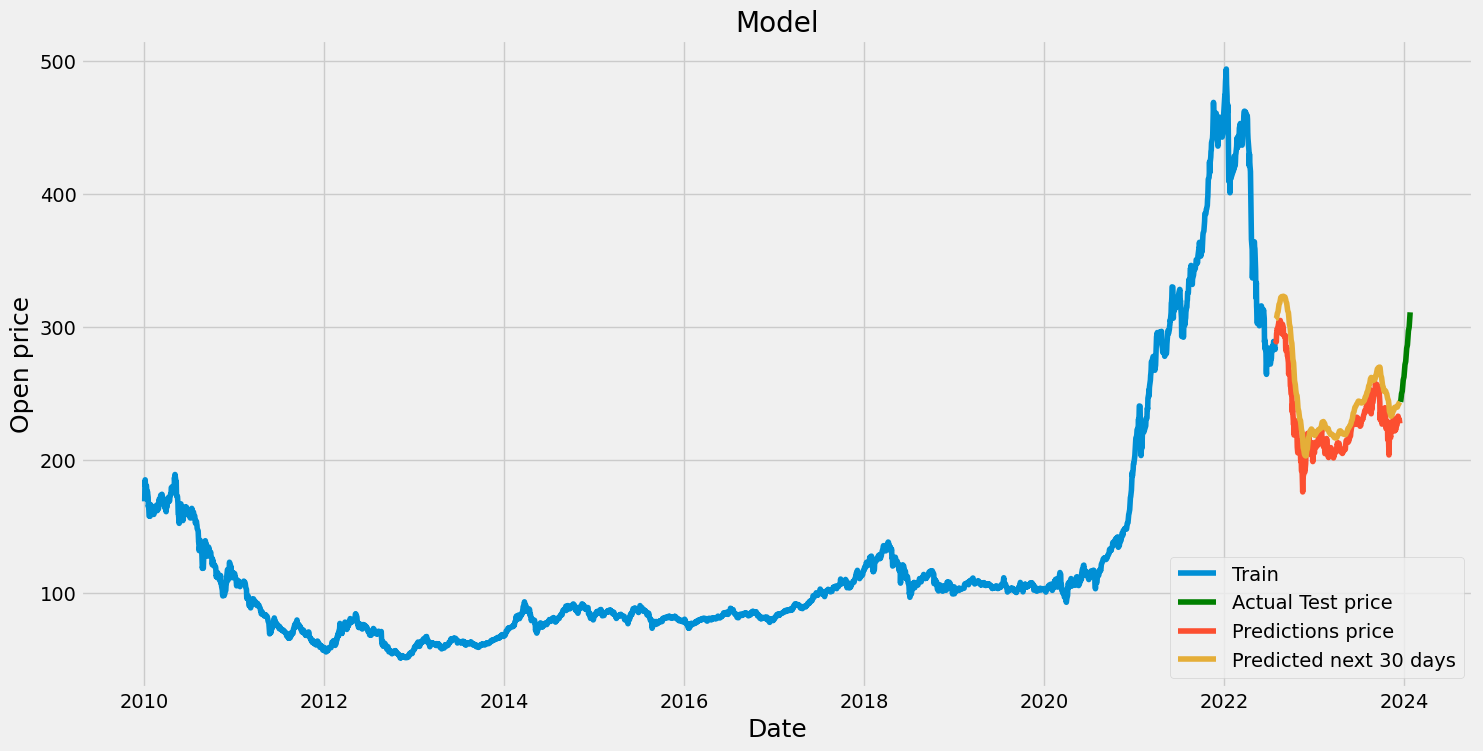
\includegraphics[width=0.8\linewidth]{LSTM-HNX-91.png}
    \caption{The LSTM best modal for HNX-Index}
    \label{fig:example}
\end{figure}

\subsubsection{SEQ2SEQ}
\begin{table}[H]
    \centering
    \begin{tabular}{|c|c|c|}
        \hline
         Measurement & Ratio &  Result  \\
        \hline
             & \textbf{7-3} & \textbf{0.95} \\
        MAE  & 8-2 & 1.05  \\
            & 9-1 & 2.03 \\
        \hline
           &\textbf{ 7-3 }& \textbf{2.00}  \\
        MSE  & 8-2 & 2.65 \\
            & 9-1 & 9.47  \\
        \hline
           & \textbf{7-3} & \textbf{1.41} \\
        RMAE  & 8-2 & 1.62  \\
            & 9-1 & 3.07 \\
        \hline
           &\textbf{ 7-3} & \textbf{0.01}  \\
        MAPE  & 8-2 & 0.10  \\
            & 9-1 & 0.01 \\
        \hline
    \end{tabular}
    \label{table:example}
\end{table}
\begin{figure}[H]
    \centering
    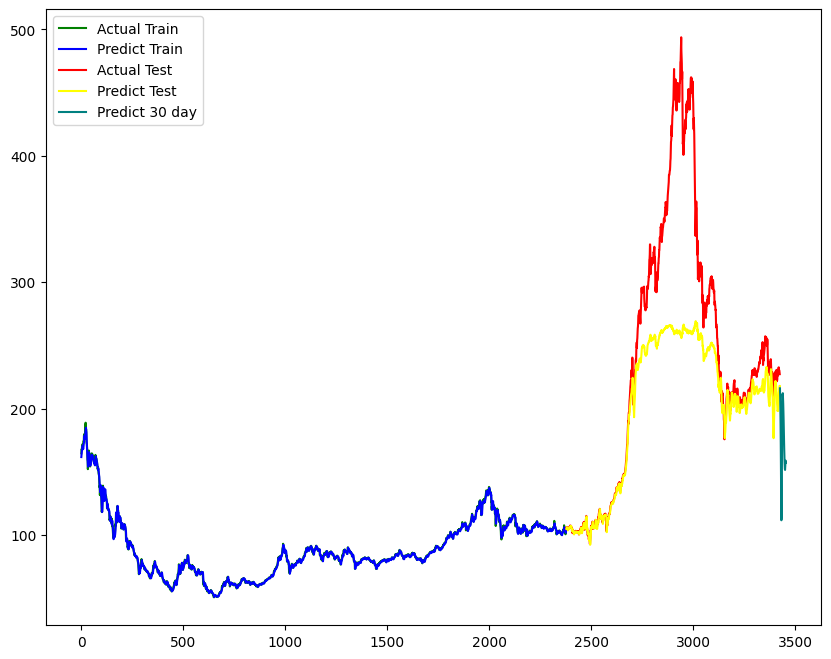
\includegraphics[width=0.8\linewidth]{RE HNX 73.jpg}
    \caption{The SEQ2SEQ best modal for HNX-Index}
    \label{fig:example}
\end{figure}

% ======
\subsection{UPCOM-Index}
\subsubsection{Linear regression}
\begin{table}[H]
    \centering
    \begin{tabular}{|c|c|c|}
        \hline
         Measurement & Ratio &  Result  \\
        \hline
             & 7-3 & 17.76 \\
        MAE  & 8-2 & 24.39  \\
            & \textbf{9-1} & \textbf{5.88} \\
        \hline
           & 7-3 & 802.04  \\
        MSE  & 8-2 & 767.56 \\
            & \textbf{9-1} & \textbf{49.70}  \\
        \hline
           & 7-3 & 22.40 \\
        RMAE  & 8-2 & 27.70  \\
            & \textbf{9-1} & \textbf{7.04} \\
        \hline
           & 7-3 & 19.98  \\
        MAPE  & 8-2 & 25.74  \\
            & \textbf{9-1} & \textbf{7.19} \\
        \hline
    \end{tabular}
    \label{table:example}
\end{table}
\begin{figure}[H]
    \centering
    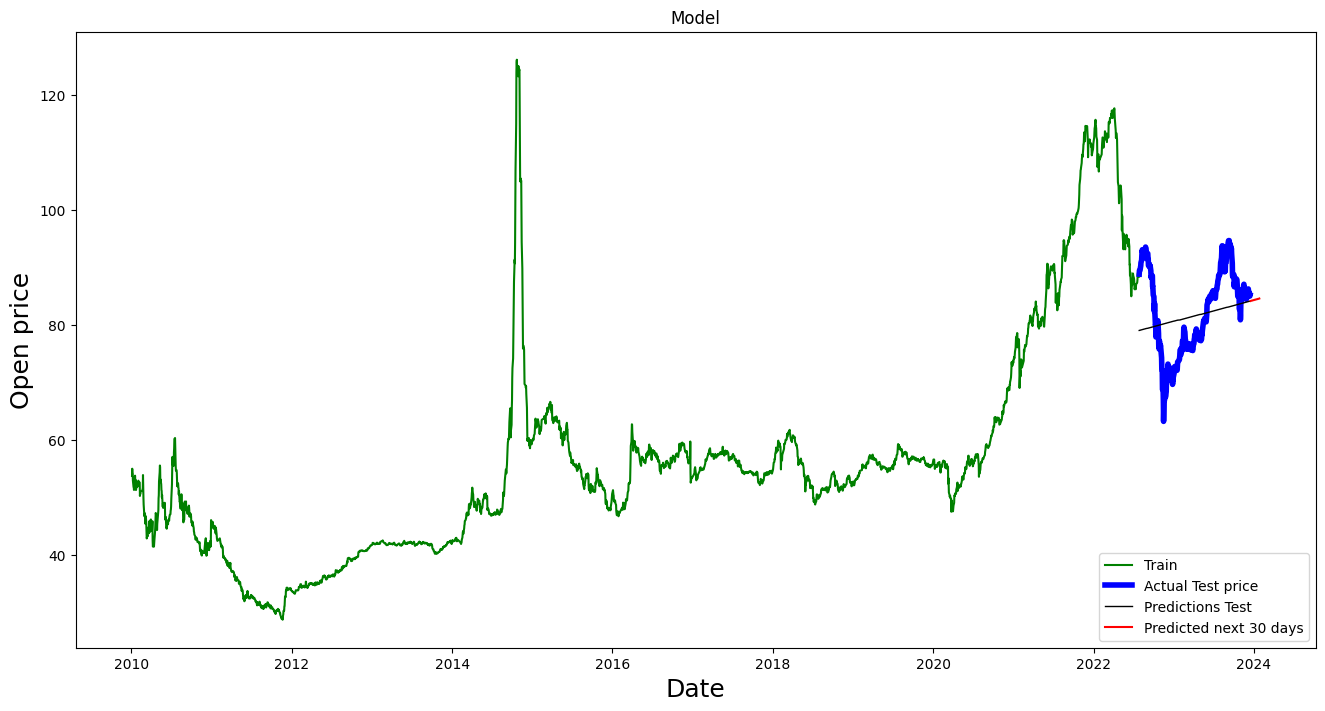
\includegraphics[width=0.8\linewidth]{LINEAR UPCOM 91.jpg}
    \caption{The Linear Regression best modal for UPCOM-Index}
    \label{fig:example}
\end{figure}

\subsubsection{ARIMA}
\begin{table}[H]
    \centering
    \begin{tabular}{|c|c|c|}
        \hline
         Measurement & Ratio &  Result  \\
        \hline
             & \textbf{7-3} & \textbf{0.54}  \\
        MAE  & 8-2 & 0.62  \\
            & 9-1 & 0.54  \\
        \hline
           & \textbf{7-3} & \textbf{0.67}  \\
        MSE  & 8-2 & 0.80  \\
            & 9-1 & 0.67  \\
        \hline
           & \textbf{7-3} & \textbf{0.81}  \\
        RMAE  & 8-2 & 0.89  \\
            & 9-1 & 0.81  \\
        \hline
           & \textbf{7-3} & \textbf{0.00}  \\
        MAPE  & 8-2 & 0.00  \\
            & 9-1 & 0.00  \\
        \hline
    \end{tabular}
\begin{figure}[H]
    \centering
    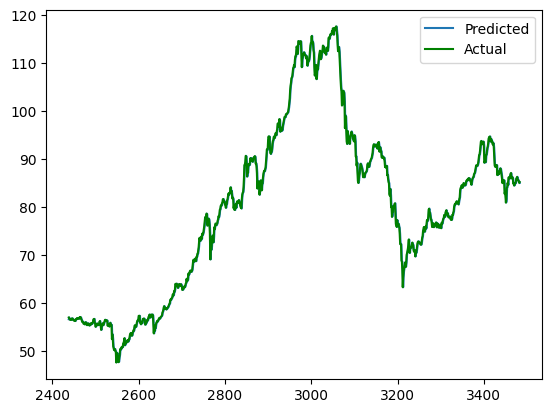
\includegraphics[width=0.8\linewidth]{ARIMA-UPC-73.png}
    \caption{The ARIMA best modal for Upcom-index}
    \label{fig:example}
\end{figure}

    \label{table:example}
\end{table}

\subsubsection{GRU}
\begin{table}[H]
    \centering
    \begin{tabular}{|c|c|c|}
        \hline
         Measurement & Ratio &  Result  \\
        \hline
             & 7-3 & 80.98  \\
        MAE  & 8-2 &  89.92 \\
            & \textbf{9-1} & \textbf{81.94}  \\
        \hline
           & 7-3 & 6824.94  \\
        MSE  & 8-2 & 8245.04  \\
            & \textbf{9-1} & \textbf{6755.17}  \\
        \hline
           & 7-3 & 82.61  \\
        RMAE  & 8-2 & 90.00  \\
            & \textbf{9-1} & \textbf{82.18}  \\
        \hline
           & 7-3 & 154.55  \\
        MAPE  & 8-2 & 143.42  \\
            & \textbf{9-1} & \textbf{148.71}  \\
        \hline
    \end{tabular}
    \label{table:example}
\end{table}
\begin{figure}[H]
    \centering
    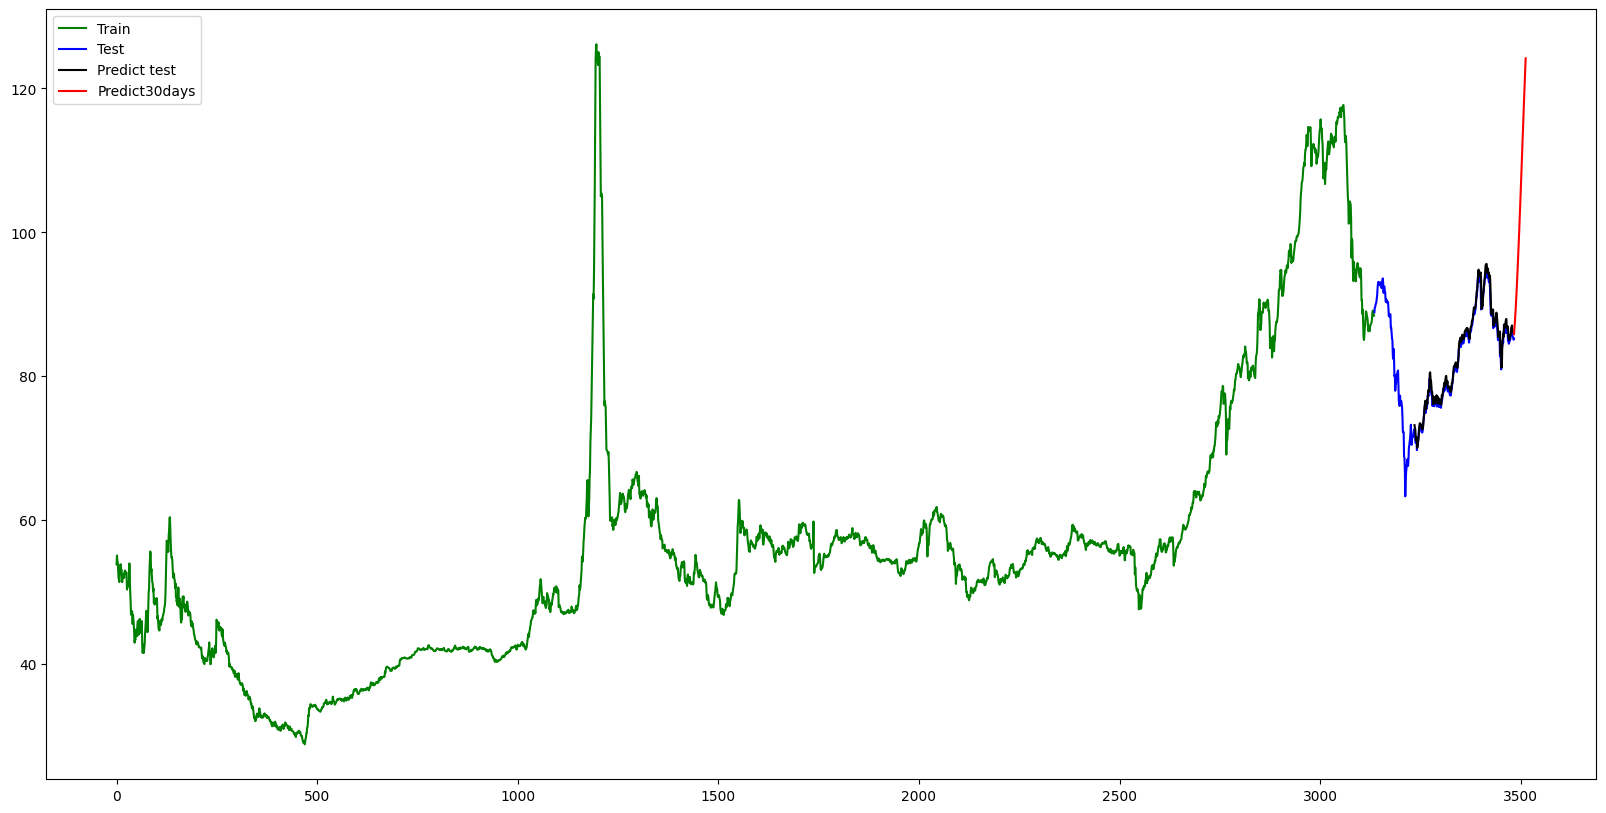
\includegraphics[width=0.8\linewidth]{GRU-UPC-91.png}
    \caption{The GRU best modal for UPCOM-Indes}
    \label{fig:example}
\end{figure}
\subsubsection{SVR}
\begin{table}[H]
    \centering
    \begin{tabular}{|c|c|c|}
        \hline
         Measurement & Ratio &  Result  \\
        \hline
             & 7-3 & 12.01 \\
        MAE  & 8-2 & 14.76  \\
            & \textbf{9-1} &\textbf{ 0.26} \\
        \hline
           & 7-3 & 315.60  \\
        MSE  & 8-2 & 396.99 \\
            & \textbf{9-1} & \textbf{0.12}  \\
        \hline
           & 7-3 & 17.76 \\
        RMAE  & 8-2 & 19.92  \\
            & \textbf{9-1} & \textbf{0.35} \\
        \hline
           & 7-3 & 0.12  \\
        MAPE  & 8-2 & 0.14  \\
            & \textbf{9-1} & \textbf{0.00} \\
        \hline
    \end{tabular}
    \label{table:example}
\end{table}
\begin{figure}[H]
    \centering
    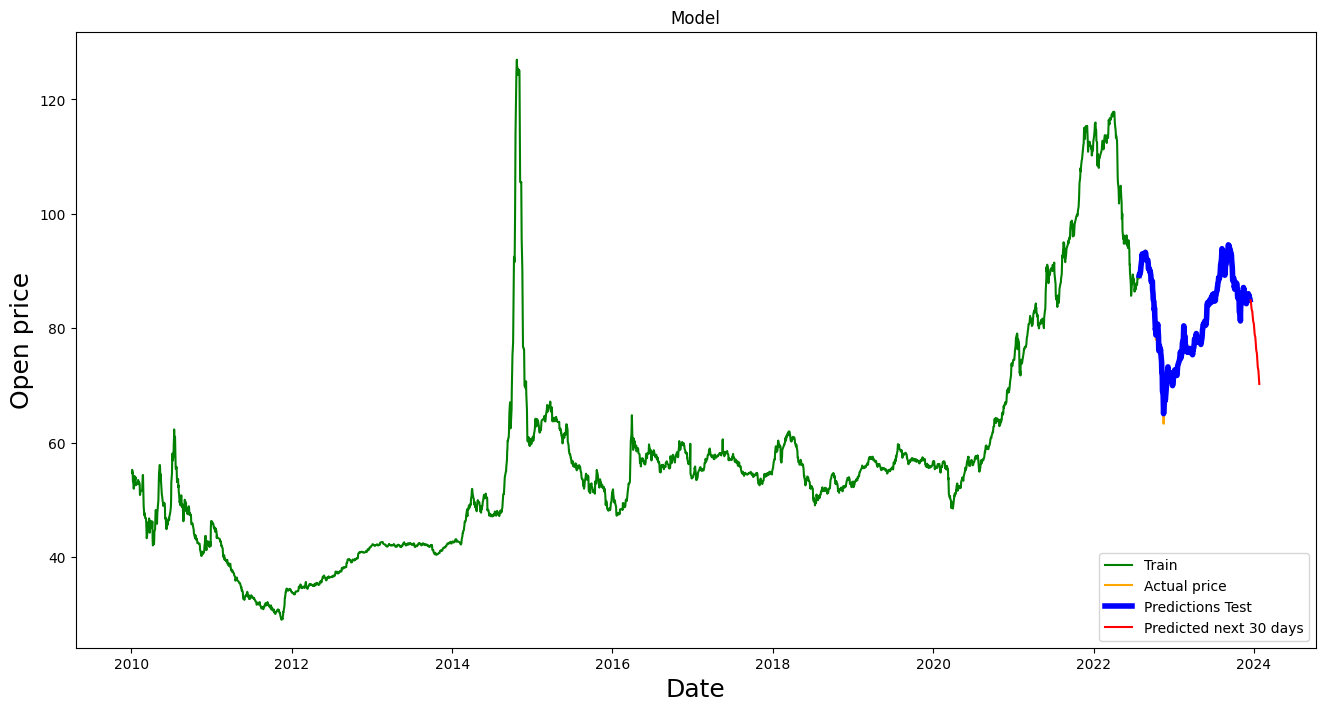
\includegraphics[width=0.8\linewidth]{SVR UPCOM 91.jpg}
    \caption{The SVR best modal for UPCOM-Index}
    \label{fig:example}
\end{figure}

\subsubsection{LSTM}
\begin{table}[H]
    \centering
    \begin{tabular}{|c|c|c|}
        \hline
         Measurement & Ratio &  Result  \\
        \hline
             & 7-3 & 8.31  \\
        MAE  & 8-2 & 12.03  \\
            & \textbf{9-1} &\textbf{ 7.00}  \\
        \hline
           & 7-3 & 132.24  \\
        MSE  & 8-2 & 235.75  \\
            & \textbf{9-1} & \textbf{79.80}  \\
        \hline
           & 7-3 & 11.49  \\
        RMAE  & 8-2 & 15.35  \\
            & \textbf{9-1} & \textbf{8.93}  \\
        \hline
           & 7-3 & 0.09  \\
        MAPE  & 8-2 & 0.12  \\
            & \textbf{9-1} & \textbf{0.08}  \\
        \hline
    \end{tabular}
    \label{table:example}
\end{table}
\begin{figure}[H]
    \centering
    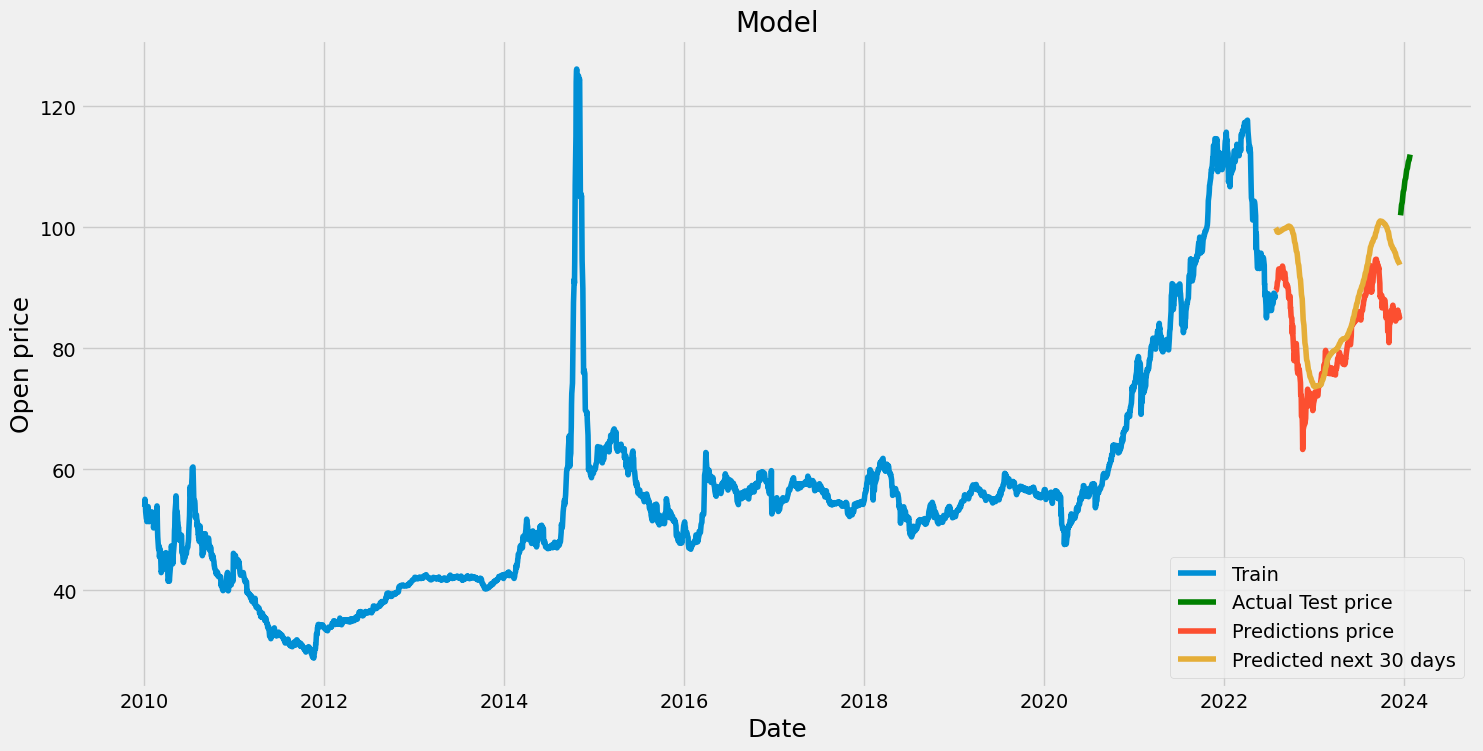
\includegraphics[width=0.8\linewidth]{LSTM-UPC-91.png}
    \caption{The LSTM best modal for UPCOM-Index}
    \label{fig:example}
\end{figure}


\subsubsection{SEQ2SEQ}
\begin{table}[H]
    \centering
    \begin{tabular}{|c|c|c|}
        \hline
         Measurement & Ratio &  Result  \\
        \hline
             & \textbf{7-3} & \textbf{0.40} \\
        MAE  & 8-2 & 0.51  \\
            & 9-1 & 0.45 \\
        \hline
           & \textbf{7-3} &\textbf{ 0.41}  \\
        MSE  & 8-2 & 0.56 \\
            & 9-1 & 0.53  \\
        \hline
           & \textbf{7-3} & \textbf{0.64} \\
        RMAE  & 8-2 & 0.74  \\
            & 9-1 & 0.72 \\
        \hline
           & \textbf{7-3} & \textbf{0.00}  \\
        MAPE  & 8-2 & 0.01  \\
            & 9-1 & 0.00 \\
        \hline
    \end{tabular}
    \label{table:example}
\end{table}
\begin{figure}[H]
    \centering
    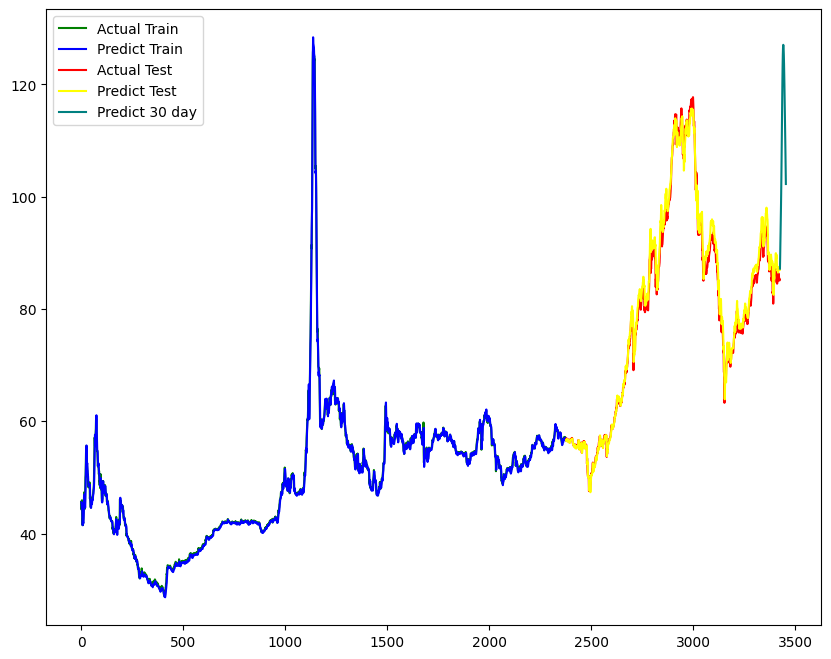
\includegraphics[width=0.8\linewidth]{SE UPC 73.jpg}
    \caption{The SEQ2SEQ best modal for UPCOM-Index}
    \label{fig:example}
\end{figure}

\section{CONCLUSION}
In conclusion, the statistical analysis reveals a clear superiority of the SEQ2SEQ algorithm over its counterparts. When applied to VNI data with a 7-3 ratio, SEQ2SEQ demonstrated remarkable results, achieving an MAE of 6.3, MAPE of 0.1, and RMAE of 9.1. Similarly, in the case of HNXIndex data, SEQ2SEQ with a 7-3 ratio showcased impressive figures, including an MAE of 0.95, MAPE of 0.1, and RMAE of 1.41. Moreover, when tested on UPC data, the SEQ2SEQ model with a 7-3 ratio achieved an outstanding performance with an MAE of 0.40, MAPE of 0.0, and RMAE of 0.64.

The SEQ2SEQ algorithm's exceptional forecasting capabilities can be attributed to its utilization of SEQ2SEQ-LSTM, where both the Encoder and Decoder employ multiple layers of LSTM modal to learn and identify Context Vector. This ensures that all crucial information is effectively retained in the forecasting process. The robust results obtained across different datasets underscore the reliability and effectiveness of SEQ2SEQ in predictive modeling.

\section{Future Research Directions}
In our prospective research, the focus lies on elucidating the intricate dynamics of algorithmic synergy. The systematic exploration aims to uncover the nuanced interactions within collaborative algorithms, particularly in the context of the amalgamation "Random Forest + XG-Boost + LSTM." The anticipation stems from the prospect of unveiling a composite solution that not only amalgamates the unique strengths of each algorithm but also augments our predictive capabilities, rendering the system more adaptable and robust.

In future trajectory, a specific emphasis is placed on immersing ourselves in the complexities of high-complexity algorithms, promising intricate analyses for heightened precision in predictive outcomes. The objective is not solely the utilitarian application of these advanced tools but, significantly, a comprehensive understanding of their underlying mechanisms. This comprehension forms the bedrock of our pursuit for enhanced accuracy and insight within the dynamic milieu of stock market forecasting.
\section{ACKNOWLEDGEMENT}
I would like to express my heartfelt gratitude to Associate Professor Dr. Nguyen Dinh Thuan and Mr. Nguyen Minh Nhut for their wholehearted dedication and invaluable assistance throughout my academic journey. Their unwavering support, guidance, and encouragement have played a pivotal role in shaping my understanding and enhancing my knowledge in the field. I am truly fortunate to have had the opportunity to work with such dedicated mentors, and I am sincerely thankful for their contributions to my academic and personal development.

\bibliographystyle{IEEEtran}
\bibliography{bibliography/mybibfile}

%% these lines used to import a separate ".bib" for the bibliografy.


%% UNCOMMENT these lines below (and remove the 2 commands above) if you want to embed the bibliografy.
% \begin{thebibliography}{00}
% \bibitem{b1} 
% \end{thebibliography}
%%%%%%%%%%%%%%%
\EOD

\end{document}
